\documentclass[11pt,paper=a4,parskip=half]{scrartcl}
\usepackage[utf8]{inputenc}
\usepackage[T1]{fontenc}

\newcommand\documenttitle{SWP Internet Communikation: Report}
\newcommand\pdftitle{\documenttitle}

\usepackage{lmodern}
\usepackage{mathtools,amssymb,amsthm}
\usepackage[english]{babel}
\usepackage[cmyk]{xcolor}
%\usepackage{tikz}
%\usepackage{nicefrac}
\usepackage[margin=2cm,top=3cm,headheight=30pt,voffset=10pt]{geometry}
\usepackage{setspace}
\usepackage{fancyhdr}
\usepackage{lastpage}
\usepackage{verbatim}
%\usepackage[european]{circuitikz}
%\usepackage{siunitx}
\usepackage{placeins} % \FloatBarrier
\usepackage{float}
%\usepackage{dcolumn}
\usepackage{tabu}
\usepackage{booktabs}
\usepackage[inline]{enumitem}
\usepackage{microtype}
\usepackage[bf]{caption}
\usepackage[pdftex]{adjustbox}
\usepackage[pdftitle={\pdftitle},pdfborder={0 0 0}]{hyperref}
\usepackage[fixlanguage]{babelbib}
\usepackage{xfrac}
\usepackage{etoolbox}
\usepackage{pdfpages}

%%%%  TEXT  %%%%

% text formatting
\addtokomafont{disposition}{\rmfamily}
\addtokomafont{descriptionlabel}{\rmfamily\bfseries}
\setcounter{secnumdepth}{0} % no heading numeration
\RedeclareSectionCommand[beforeskip=.5\baselineskip,afterskip=.25\baselineskip]{subsubsection}
\RedeclareSectionCommand[beforeskip=.3\baselineskip]{paragraph}
\captionsetup{format=plain}

% helpers
\newcommand\http[1]{\href{http://#1}{#1}}
\newcommand\https[1]{\href{https://#1}{#1}}

\makeatletter
% fix spacing within minipage  (https://tex.stackexchange.com/a/141123/73880)
\newlength{\currentparskip}
\setlength{\currentparskip}{\parskip}
\newcommand{\@minipagerestore}{\setlength{\parskip}{\currentparskip}}
% fix spacing around verbatim  (https://tex.stackexchange.com/a/43336/73880)
\preto{\@verbatim}{\topsep=0pt \partopsep=0pt }
\makeatother

%%%%  MATH  %%%%

\DeclareCollectionInstance{betterkern}{xfrac}{mathdefault}{math}{slash-right-mkern=-2.5mu}  \UseCollection{xfrac}{betterkern}
\DeclareSymbolFont{largesymbols}{OMX}{cmex}{m}{n} % widehat tex.sx/q/219353/73880

% fix spacing around \left/\right (https://tex.stackexchange.com/a/2610/73880)
\let\originalleft\left
\let\originalright\right
\renewcommand{\left}{\mathopen{}\mathclose\bgroup\originalleft}
\renewcommand{\right}{\aftergroup\egroup\originalright}

% units
\makeatletter\@ifpackageloaded{siunitx}{
\sisetup{per-mode=fraction,fraction-function=\tfrac,
         output-decimal-marker={,},
         exponent-product=\mathop{\!\cdot\!},
         inter-unit-product=\mathop{\!\cdot\!},
         table-number-alignment=right}
\newcommand\IS[2]{\SI{#2}{#1}}
\newcommand\s{\IS{\second}}
\newcommand\mm{\IS{\milli\meter}}
\newcommand\nr{\IS{}}
}{}\makeatother

%%%%  PAGE  %%%%

\pagestyle{fancy} \fancyhf{}
\chead{Garcia\,·\,Ihrig\,·\,Sigler\,·\,Zaboub  \hfill
    \textbf{\documenttitle}  \hfill
    page \thepage\,/\,\pageref*{LastPage}}



\begin{document}


\thispagestyle{empty}


\begin{center}

\begin{spacing}{1.2}
\textbf{ \LARGE
Albert Garcia \\
Jannis Ihrig \\
Marian Sigler \\
Manar Zaboub \\
}

\end{spacing}\vspace{2.5em}


\textbf{ \Huge Software Project \\ \emph{Internet Communication} \\\vspace{0.8em}
Final Report}
\vspace{2.5em}

\begin{spacing}{1}
\Large

FU Berlin, Summer Term 2018

Prof. Dr. Matthias Wählisch
\end{spacing}
\end{center}

\vspace{10mm}


\setcounter{tocdepth}{2}
\tableofcontents

\newpage



%%%%%%%%%%%%%%%%%%%%%%%%%%%%%%%%%%%%%%%%%%%%%%%%%%%%%%%%%%%%%%%%%%%%%%
\section{Introduction}






%%%%%%%%%%%%%%%%%%%%%%%%%%%%%%%%%%%%%%%%%%%%%%%%%%%%%%%%%%%%%%%%%%%%%%
\section{Use Case}
\label{sec:usecase}

  In the following section we describe the scope of application for which our application was build for.

  We assume several seperate planter pots are given. These can have some distance between each other but are located in one general location.

  The application to build should allow to monitor the humitidy of each single planter pot separately and remotely, e.g. from a computer indoors. The parts of the system responsible for humidity monitoring, i.e. sensor nodes, should be easy to install, require low maintenance and so be able to remain with the planter pots or inside the soil for long periods of time. As an extra prerequisite specific to the course, we were asked to use the Atmel \textit{SAM R21 Xplained Pro} MCU (SAMR21 in the following) as hardware for the sensor nodes.  Additionally, these Atmel MCUs should run \textit{RIOT} as their operating system.

  Additinally to humidity monitoring, the system should take care of watering the planter pots automatically.

\section{Planning}
\subsection{Planned Solution}
  \paragraph{Sensor and pump control nodes} To measure humidity of the single
  planter pots, we decided to use the SAMR21 MCUs as sensor nodes which should
  run the RIOT operating system. These should therefore each be equipped with
  an external humidity sensor to measure soil moisture. We regarded the
  integration of addidional sensors as temperature, light or air humidity
  sensors as desirable but not a central part of the project. We also planned
  for the possibility of multi-hop routing between the sensor nodes to increase
  the maximum range in which they can be placed.

  Additinally to monitoring purposes, one central goal described in the section
  \textit{Use Case} was to water the planter pots. We therefore decided  to
  introduce an additinal node which should collect all sensor data and control
  a water pump. When turned on, the pump should water all plants collectively
  to simplify the setup.

  The decision of using the SAMR21 as sensor nodes and pump controller had a
  big impact on the planned system architecture, as it has a low power
  consumption and offers wireless connectivity via 6LoWPAN over IEEE802.15.4.
  Together, this should increase battery lifetime and reduce the need for
  maintenance, as was one of our set goals.

  \paragraph{Gateway node and web frontend} Another node should receive data
  from the pump control node and publish it to a web server under our control.
  It therefore had to be able to connect to the local network via Ethernet or
  WiFi based on IEEE802.11. A web frontend should then allow to monitor all
  sensor data remotely.

\subsection{Milestones}



%%%%%%%%%%%%%%%%%%%%%%%%%%%%%%%%%%%%%%%%%%%%%%%%%%%%%%%%%%%%%%%%%%%%%%
\section{Implementation}

\subsection{Planning and General Overview}

The general plan for the system architecture was derived in the first two weeks from the given task described in the section \textit{Use Case}.

sensor nodes that measure humidity (and possibly other sensor data) and send it to one central collector node. Use SAMR21. Extend with a moisture sensor to measure soil humidity. Also possible to send temp over network. Also generally possible to use the ... PhyNode that has an extended array of sensors.

One main factor were the given SAMR21 MCUs and their capability to comminicate via 6LoWPAN over IEEE 802.15.4. As multiple sensor nodes would be distributed over different planter pots,

multihop

One central location that acts as a gateway to the internet. This node needs a ethernet or regular wifi connection. Therefore not SAMR21 but raspberry pi with a 6LoWPAN usb dongle.

One webserver that serves the status (humidity) of the sensor nodes.

to be able to water, node that controls some water supply. To simplify the case, we assumed one node to controle a pump that would water all plants at the same time.

As pump controller needs to monitor all sensor nodes anyway to make the decision if the pump should be opened, the aggregation of all sensor data falls together with the node that controls the pump.

Planned system split into different components

Split into 3 Milestones



  The use of the \textit{samr21-xrpo} was given as an additional prerequisite.
  \begin{figure}[h]
    \centering
    % \def\svgwidth{\columnwidth}
    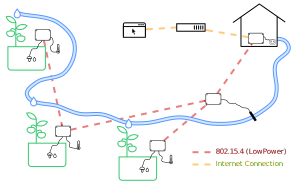
\includegraphics[scale=0.3]{schema}
	  \caption{Overview of the general system architecture resulting from the analysis of the given task described in the previous section.}
    \label{fig:schema}
  \end{figure}


%%%%%%%%%%
\subsection{Sensors}
\label{sec:sensors}

The central task of the

%%%%%%%%%%
\subsection{Network}



%%%%%%%%%%
\subsection{H2O Protocol}



%%%%%%%%%%
\subsection{Pump Control}

The Pump Control is the set of algorithms that manage the water pump.
In this subsection we present the functions that are being used and the reason of the developing of these functions.

First of all we have to present the design of the pump controller, in this case we have implemented a threshold system which allows the controller to decide the next action of the pump. As we have two types of sensors (the one that controls the water level of the pump and the rest) there are two types of thresholds with different values that are defined after a couple of practical tests.

Once the design is presented we can start to describe the different functions that are used in the pump control.

Function: reset\_table( int table[~][~])

This function  fills the bidimensional array of 0 and also set to 0 different variables.

The function is used when the pump changes of state(open or close) or when all the normal sensors (the ones not in water) had sended data.

Function: print\_table (int table[~][~])

This function prints in the console the ID, the last value received and the time when the value was received of each sensor stored in the table.
The function is used to control the correct functioning of the table and of the algorithm and to control that the pump is receiving the correct values of the different sensors.
It is a purely informative function.

Function: initialize\_pump()

This function is used to initialize the GPIO that allows us to control the pump through the samr21 board.

The function calls some GPIO functions needed to initialize the GPIO and sets it low because we assume that when we start the system, the plants do not need water.

Function: make\_pump\_close()

This function closes the pump, when the algorithm calls this function had already checked that the plants have enough water and the pump is still on or the opening time has been exceeded.

To close the pump the function sets the GPIO to low using the GPIO function gpio\_clear.

Function: make\_pump\_open(int aux)

This function opens the pump, when the algorithm calls this functions had already cheacked that the plants need water and the pump is closed. The pump is opened for a concrete amount of time defined by the variable aux and then calls the function make\_pump\_close() to close the pump.

To open the pump the function sets the GPIO to high using the GPIO function gpio\_set.

Function: water\_level\_sensor\_control (int data)

This function is used to avoid the malfunctioning of the pump caused by the lack of water. If the data sended by the water sensor indicates that the water level is under a concrete threshold the function calls the function make\_pump\_close.

Function: add\_data\_table(int id, int data)

This function add to the table the data recieved from the sensors. First of all the function checks if there is existing data of this sensor already in the table, if they exist the function updates the value, if not it add a new line to the table with the new data and the actual time; finally the function calls print\_table to show the new state of the table.

Function: add\_pid\_controller(int data)

This function is used to adjust the time that the pump is open, to determine that time a set of algorithms are used that take into account the rest of the values received from the other sensors and depending on the distance between them and with the thresholds, the opening time of the pump is defined.

Function add\_set\_data(int id,int data)

This function decides if the pump should open or not, in order to do that it compares the values sended from the sensors with a set of thresholds and decides to call make\_pump\_open, make\_pump\_close or wait for more values of more sensors, it also calls the function that controls the water level sensor if it is necessary.

Function: shell\_pump\_set\_data( int argc, char * argv[])

This function is used to control the correct functioning of the pump controller algorithm and allows the developers to call the functions without sending real data from the sensors but sending it from a console.
%%%%%%%%%%
\subsection{Gateway}



%%%%%%%%%%
\subsection{Data Presentation}



%%%%%%%%%%%%%%%%%%%%%%%%%%%%%%%%%%%%%%%%%%%%%%%%%%%%%%%%%%%%%%%%%%%%%%
\section{Conclusion}





%%%%%%%%%%%%%%%%%%%%%%%%%%%%%%%%%%%%%%%%%%%%%%%%%%%%%%%%%%%%%%%%%%%%%%

\end{document}

































